\chapter[Caso di studio]{Caso di studio}

Dopo aver descritto il modello fp-HDGM da un punto di vista matematico e metodologico, in questo capitolo esso viene applicato al fenomeno del bike sharing. L'obiettivo iniziale del caso di studio è descrivere, sia nel tempo sia nello spazio, il numero di ritiri di biciclette presso una serie di stazioni (o punti di ritiro) dislocati nel quartiere Jersey della città di New York, figura ~\ref{presentazione_Jersey_City}. Dopodiché, si vuole costruire una mappa di potenziale di mercato spaziale per capire dove conviene aprire una nuova stazione al fine di aumentare il numero di ritiri e il bacino d'utenza del servizio, tenendo conto dell'iterazione concorrenziale esistente tra le stazioni.

\begin{figure}[b!]
	\centering
	\subfigure[]{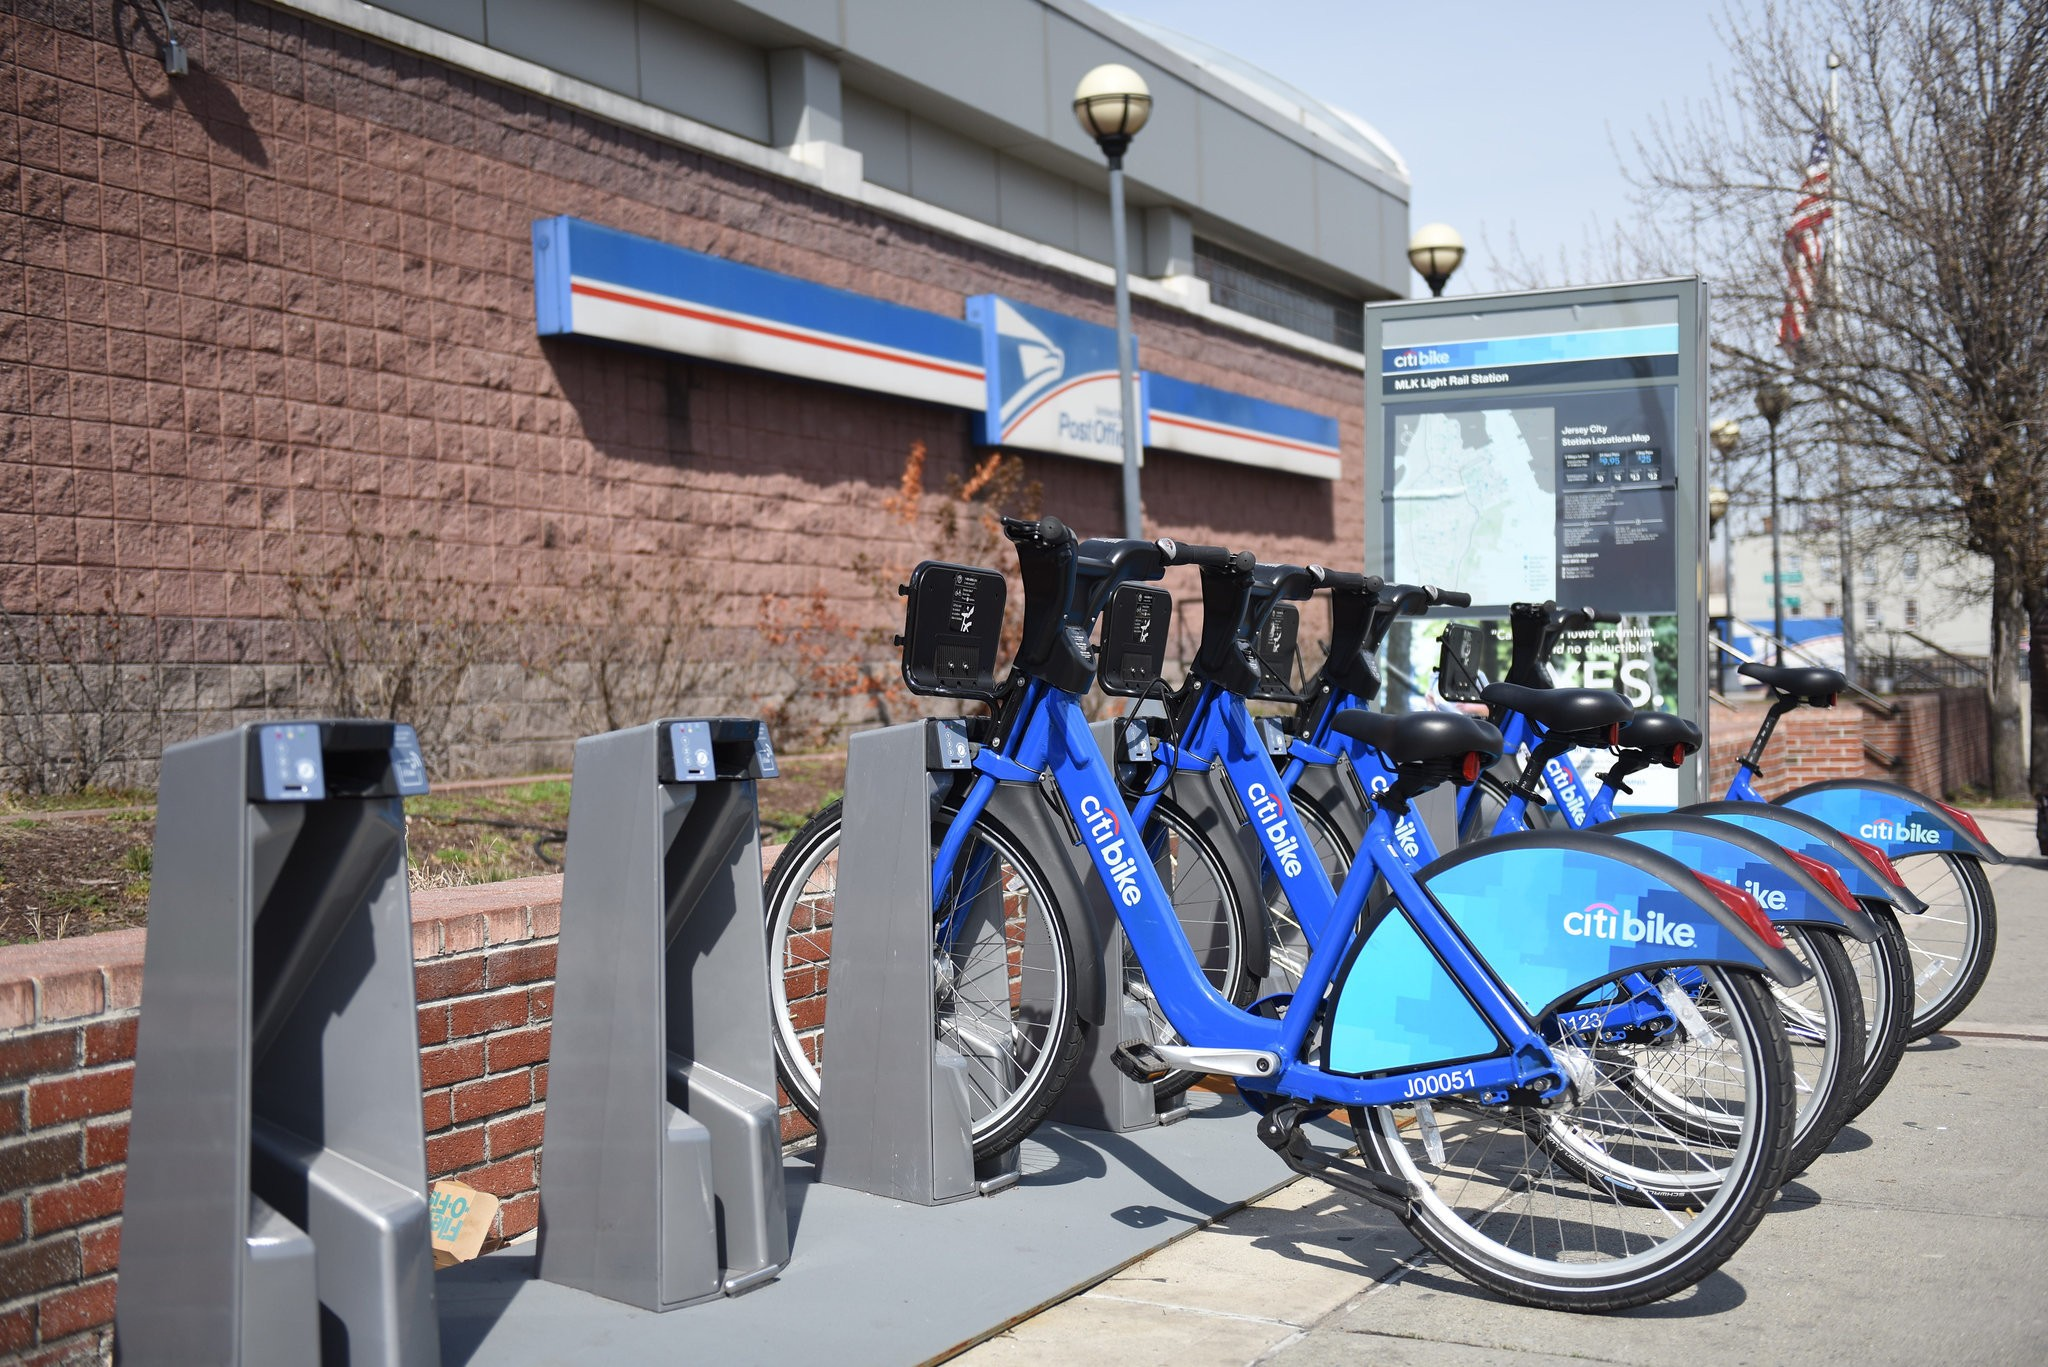
\includegraphics[height=137px]{Immagini/4. Caso di studio/Introduzione/Citi Bike}\label{Citi_Bike}}\quad
	\subfigure[]{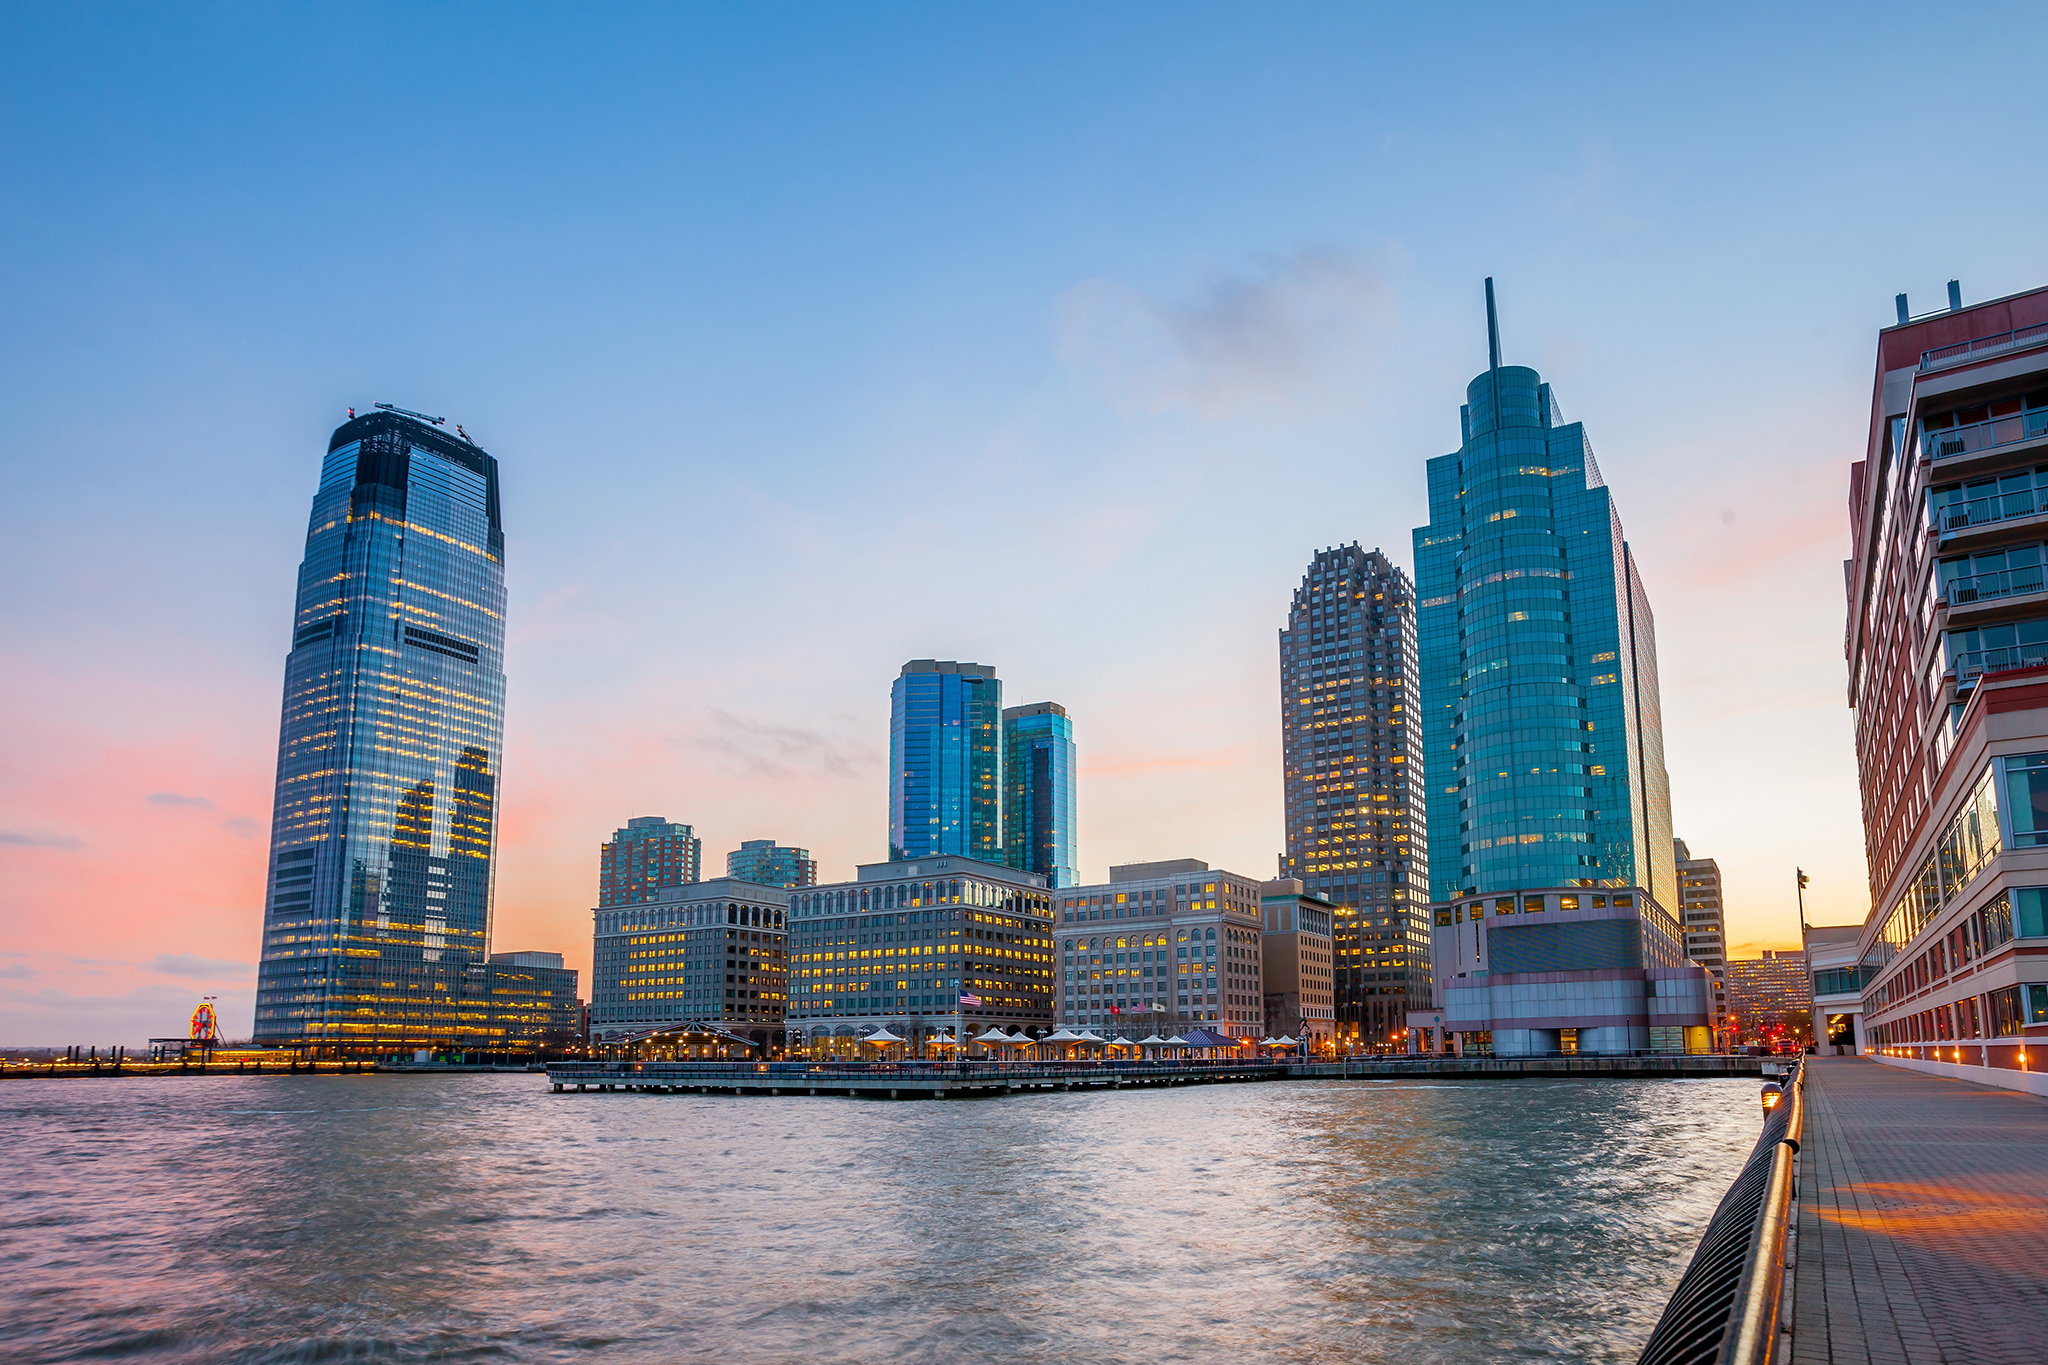
\includegraphics[height=137px]{Immagini/4. Caso di studio/Introduzione/Veduta Jersey City}\label{veduta_Jersey_City}}\quad
	\caption[Punto di ritiro delle biciclette e veduta del quartiere Jersey]{punto di ritiro delle biciclette gestito da Citi Bike (a) e veduta del quartiere Jersey, New York City (b).}
	\label{presentazione_Jersey_City}
\end{figure}

\section[Stato dell'arte]{Stato dell'arte}
Nelle città di tutto il mondo, l'inquinamento atmosferico rappresenta una sfida sempre più urgente e complessa. Samantha Burgess, Deputy Director del Copernicus Climate Change Service, ha affermato che il 2023 non solo è stato l'anno più caldo mai registrato, ma è anche il primo in cui tutti i giorni le temperature hanno fatto registrare valori superiori di almeno \SI{1}{\degreeCelsius} rispetto al periodo preindustriale~[\ref{sitografia_capitolo_4}].
\par L'aumento del traffico veicolare, in particolare, contribuisce in modo significativo alla diffusione di gas nocivi (es. CO$_2$ ed NO$_\text{X}$) e particolato nell'aria (es. PM\num{2.5} e PM\num{10}), compromettendo la salute pubblica e l'ambiente. In questo contesto, il bike sharing emerge come una soluzione innovativa e sostenibile per affrontare l'inquinamento urbano. Attraverso la condivisione delle biciclette, questo sistema offre un'alternativa efficace al trasporto privato a motore, riducendo le emissioni di gas serra, i consumi energetici e migliorando la qualità dell'aria nelle città~[\cite{paper_bike_sharing_e_ambiente}].
\par Per modellare il fenomeno del bike sharing le condizioni del tempo atmosferico risultano essere appropriate. Infatti, le variabili meteorologiche come pioggia, temperatura e vento, giocano un ruolo cruciale nel determinare la frequenza e la disponibilità delle biciclette per gli utenti, nonché la percezione stessa dell'attrattività del bike sharing come mezzo di trasporto. Inoltre, risulta interessante capire se la vicinanza di un punto di ritiro dalla più vicina fermata del treno o metropolitana incentiva l'utilizzo di quest'ultima piuttosto che della bicicletta, soprattutto in condizioni di maltempo~[\cite{paper_bike_sharing_e_meteo}].
\par In generale, anche gli aspetti urbanistici e demografici possono aiutare nella descrizione del fenomeno. Infatti, la densità abitativa, la disposizione delle infrastrutture ciclabili, la distribuzione della popolazione, la vicinanza ad alberghi e ai punti di interesse possono influenzare l'adozione della bicicletta a noleggio come mezzo di trasporto urbano~[\cite{paper_bike_sharing_e_popolazione}].
\par Infine, anche gli eventi straordinari possono avere un impatto significativo sul comportamento degli utenti e sulla dinamica del sistema. Uno di questi eventi straordinari è rappresentato dal lockdown imposto a causa della pandemia di COVID-\num{19}. Il lockdown ha comportato una serie di cambiamenti radicali nelle abitudini di spostamento delle persone, con effetti tangibili sull'utilizzo del bike sharing nelle metropoli di tutto il mondo. Pertanto, è essenziale comprendere come la chiusura obbligata abbia influenzato il fenomeno in oggetto, considerando sia gli aspetti legati alla riduzione del trasporto pubblico che quelli associati alla promozione di modalità di spostamento individuali e sicure~[\cite{paper_bike_sharing_e_covid}].
\par In questo contesto, l'impiego di un modello spazio-temporale funzionale si presenta come una soluzione promettente per catturare la dinamica complessa che governa il noleggio e scambio di biciclette. Tale famiglia di modelli consente di considerare non solo le variazioni spaziali dell'utilizzo delle biciclette all'interno di una città, ma anche come queste variazioni si evolvono nel tempo, consentendo una comprensione più approfondita dei pattern di utilizzo e dei fattori che li influenzano. Altresì, la modellazione funzionale permette di descrivere l'evoluzione oraria del numero di ritiri durante il giorno. Infatti, quest'ultimo non rimane costante nel corso della giornata, ma presenta un andamento periodico che raggiunge i propri massimi nelle ore di punta. I trend periodici, inoltre, sono influenzati dalla tipologia di giorno, ovvero feriale o weekend (figura~\ref{trend_paper_Otto}), quindi tenere in considerazione quest'aspetto nella modellazione è fondamentale~[\cite{paper_bike_sharing_Otto}].

\begin{figure}[htpb]
	\centering
	\subfigure[]{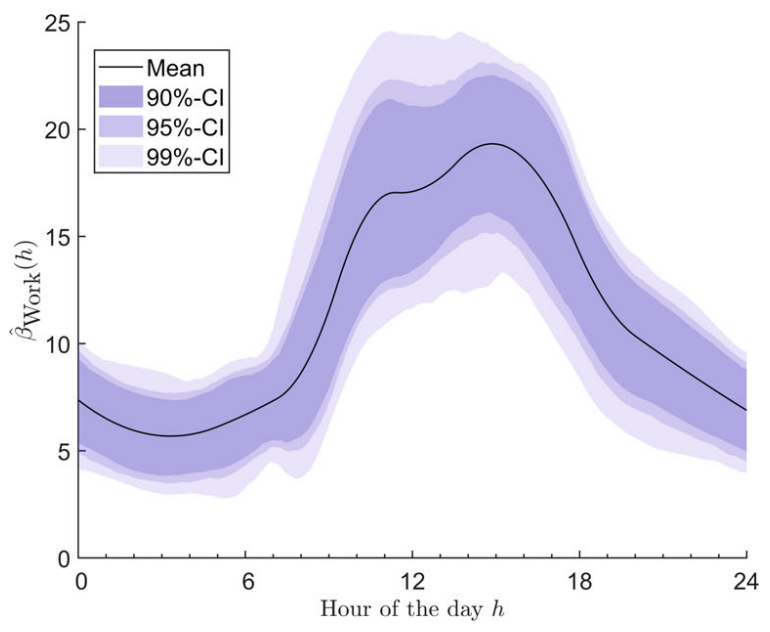
\includegraphics[height=156px]{Immagini/4. Caso di studio/Stato dell'arte/Trend_feriale}\label{trend_feriale}}\quad
	\subfigure[]{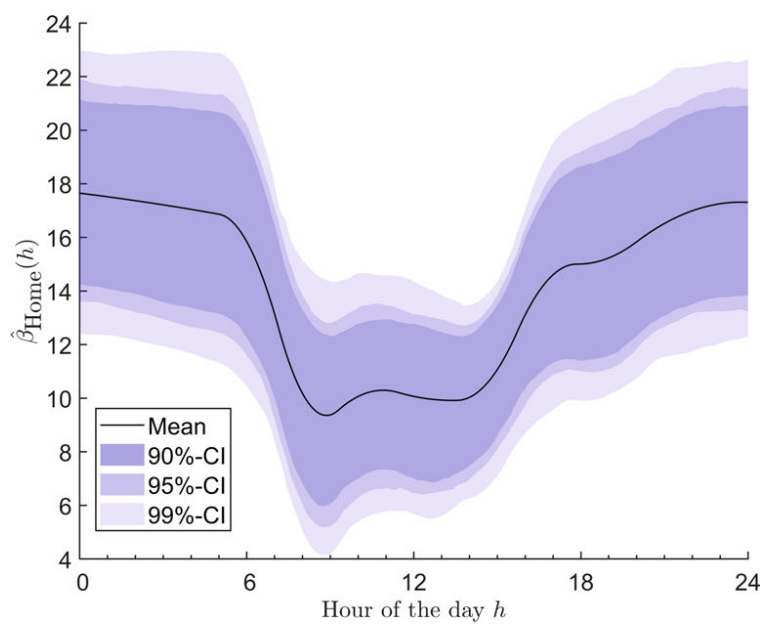
\includegraphics[height=156px]{Immagini/4. Caso di studio/Stato dell'arte/Trend_festivo}\label{trend_festivo}}\quad
	\caption[Confronto tra l'andamento orario del numero medio di ritiri nei giorni feriali e nei weekend a Helsinki]{confronto tra l'andamento orario del numero medio di ritiri di biciclette nei giorni feriali (a) e nei weekend (b) nella città di Helsinki, Finlandia.}
	\label{trend_paper_Otto}
\end{figure}

\section[Ricerca e acquisizione dati]{Ricerca e acquisizione dei dati}
Di seguito sono riportate le sorgenti dei dati utilizzati nel caso di studio:
\begin{itemize}
	\item \textbf{dati riguardanti il bike sharing}: provengono dal sito web Kaggle~[\ref{sitografia_capitolo_4}] e contengono le informazioni sul noleggio di biciclette nel \num{2020} dell'azienda Citi Bile a Jersey City. Citi Bike è un sistema di bike sharing pubblico di proprietà privata che serve i distretti di New York City, nello specifico Bronx, Brooklyn, Manhattan e Queens, oltre a Jersey City;
	\item \textbf{dati meteorologici}: contengono le serie storiche delle variabili meteorologiche più significative per la città di New York nel \num{2020}. Il provider di questi dati è Visual Crossing~[\ref{sitografia_capitolo_4}], un fornitore che offre una vasta gamma di soluzioni per l'accesso ai dati meteorologici storici e in tempo reale, nonché per la generazione di previsioni meteo;
	\item \textbf{dati inerenti le stazioni del treno/metropolitana}: dopo aver recuperato i nomi delle stazioni del treno e della metropolitana dalla mappa dei mezzi pubblici newyorkesi~[\ref{sitografia_capitolo_4}], le loro coordinate sono state reperite tramite Google Maps;
	\item \textbf{dati demografici}: il fornitore è il SEDAC~[\ref{sitografia_capitolo_4}] (Socioeconomic Data and Applications Center), un data center che fa parte del programma Earth Observing System Data and Information System (EOSDIS) della NASA. La missione principale dell'ente è quella di fornire accesso a dati socioeconomici e ambientali globali, nonché a strumenti e risorse per facilitare la ricerca e la comprensione dei cambiamenti ambientali e delle dinamiche sociali.
	\item \textbf{dati riguardanti i giorni di festività e di lockdown}: per i primi è stato fatto riferimento al sito web OfficeHolidays~[\ref{sitografia_capitolo_4}], mentre per i secondi a Wikipedia~[\ref{sitografia_capitolo_4}].
\end{itemize}
Da sottolineare, infine, che sono state processate le sole variabili d'interesse per il caso di studio; nello specifico è stato applicato un raggruppamento su base oraria, ove necessario.

\section[Descrizione del dataset]{Descrizione del dataset}
Di seguito sono riportate e descritte le variabili che compongono il dataset utilizzato per il caso di studio. Nello specifico la variabile dipendente $y(\mathbf{s}, l, t|\mathcal{S})$ è il numero di ritiri in una data ora $l$, in uno specifico giorno $t$, presso una determinata stazione di scambio di biciclette $\mathbf{s}$. Invece, le covariate possono essere suddivise in:
\begin{itemize}
	\item \textbf{variabili meteorologiche} $\mathbf{x}_{meteo}(t)$;
	\item \textbf{variabili spaziali} $\mathbf{x}_{spazio}(\mathbf{s})$;
	\item \textbf{variabili dummy} $\mathbf{x}_{dummy}(t)$.
\end{itemize}
Per completezza:
\begin{itemize}
	\item il numero di stazioni $n$ è pari a \num{51};
	\item il numero massimo di osservazioni disponibili per il dominio funzionale (orario) è \num{24};
	\item l'analisi è stata condotta su dati facenti riferimento all'anno \num{2020}, quindi $T=366$.
\end{itemize}
Infine, nel dataset non sono presenti record mancati.

\subsection[Numero di ritiri]{Variabile dipendente}
In figura~\ref{mappe_ritiri_per_stagione} si può osservare come il numero medio di ritiri giornaliero di biciclette presso le stazioni della rete di bike sharing cambi da stagione a stagione. Questa variazione è influenzata da diversi fattori legati alle condizioni meteorologiche, agli schemi di mobilità delle persone e alle attività ricreative. In estate, quando le giornate sono più lunghe e il clima è più gradevole, si verifica un generale aumento dell'utilizzo della bicicletta, figura~\ref{mappa_ritiri_estate}; le persone sono più propense a utilizzarla per spostarsi o fare gite. In autunno, invece, il numero di noleggi diminuisce leggermente poiché le giornate diventano più corte e il clima meno favorevole, figura~\ref{mappa_ritiri_autunno}. In inverno il numero medio di ritiri giornaliero tende a essere il più basso dell'anno, figura~\ref{mappa_ritiri_inverno}; le condizioni meteorologiche avverse, come il freddo, la pioggia e la neve, rendono meno attraente l'utilizzo della bicicletta. La primavera, infine, rispecchia la straordinarietà del \num{2020}; il lockdown ha limitato gli spostamenti dei cittadini newyorkesi, quindi l'utilizzo della bicicletta ha subito un brusco calo. Da notare, inoltre, l'assenza di uniformità nell'utilizzo delle stazioni; quelle situate nel centro del quartiere Jersey vengono sfruttate maggiormente rispetto ai punti di scambio periferici.
\par Infine, l'andamento orario del numero medio di noleggi in figura~\ref{ritiri_giornalieri_orari} conferma quanto detto precedentemente. Da sottolineare anche la presenza di picchi di utilizzo in concomitanza delle ore di punta.

\begin{figure}[htpb]
	\centering
	\subfigure[]{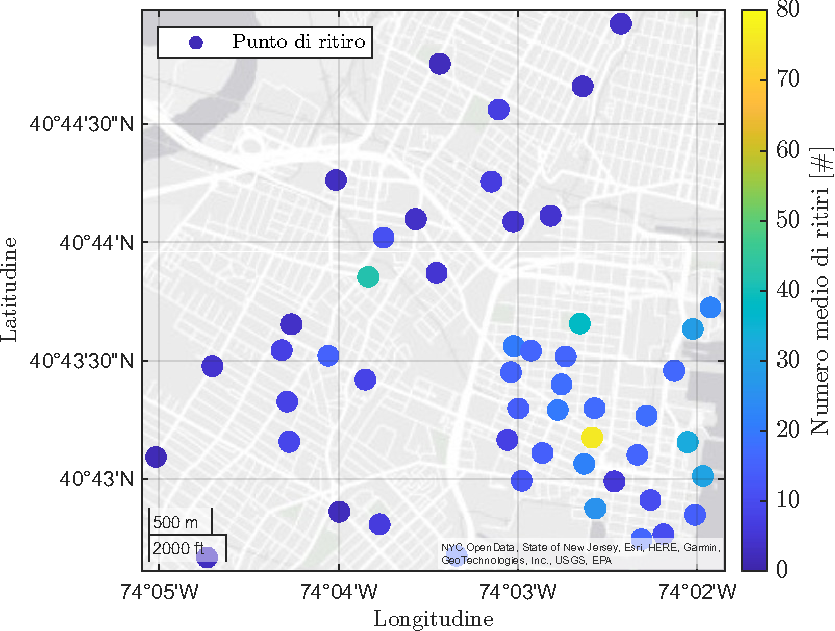
\includegraphics[height=156px]{Immagini/4. Caso di studio/Mappe/Mappa ritiri, inverno}\label{mappa_ritiri_inverno}}\quad
	\subfigure[]{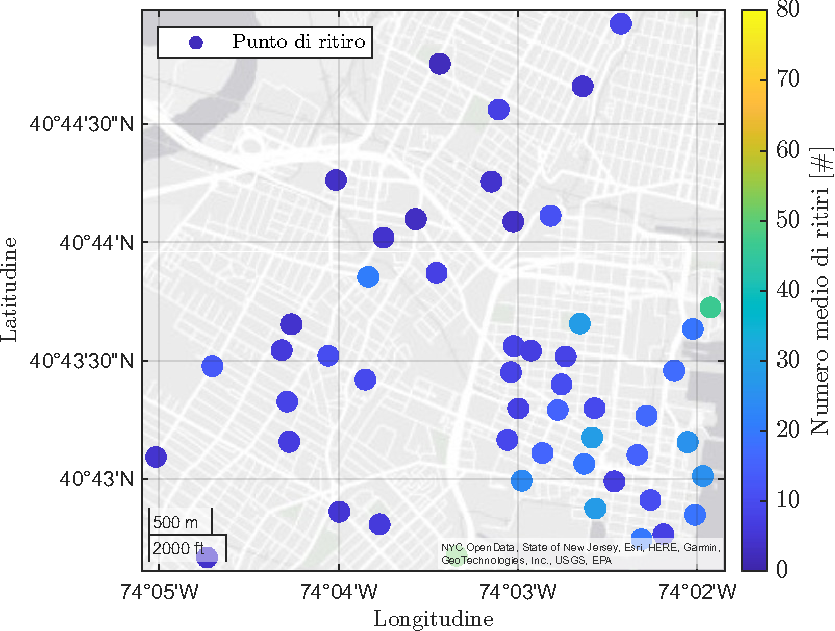
\includegraphics[height=156px]{Immagini/4. Caso di studio/Mappe/Mappa ritiri, primavera}\label{mappa_ritiri_primavera}}\quad
	\subfigure[]{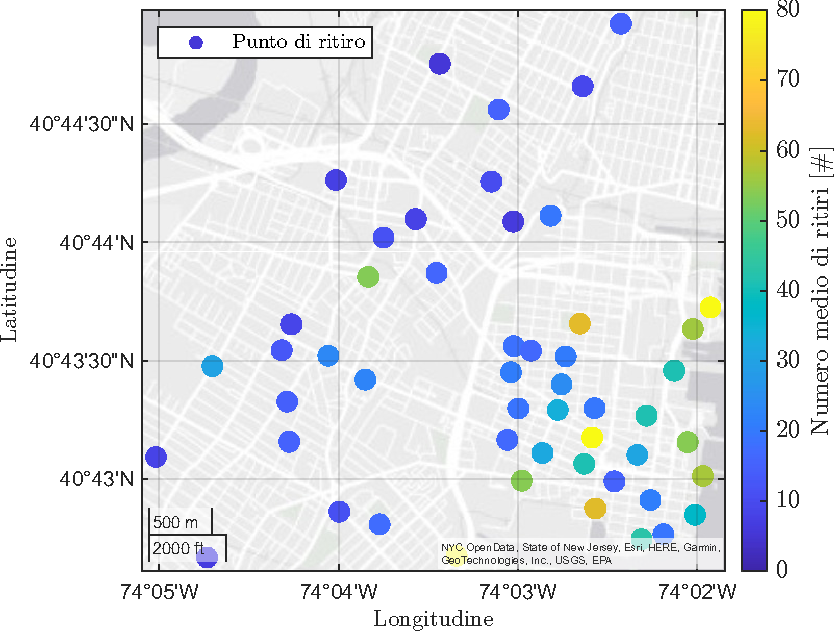
\includegraphics[height=156px]{Immagini/4. Caso di studio/Mappe/Mappa ritiri, estate}\label{mappa_ritiri_estate}}\quad
	\subfigure[]{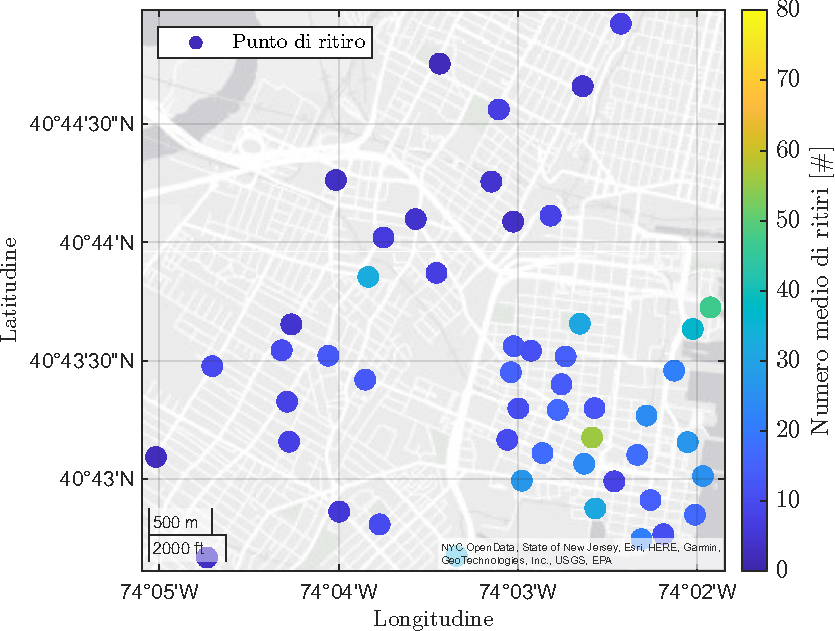
\includegraphics[height=156px]{Immagini/4. Caso di studio/Mappe/Mappa ritiri, autunno}\label{mappa_ritiri_autunno}}\quad
	\caption[Distribuzione nel numero medio di ritiri giornaliero presso le stazioni al variare della stagione]{distribuzione nel numero medio di ritiri giornaliero presso le \num{51} stazioni di scambio in inverno (a), in primavera (b), in estate (c) e in autunno (d).}
	\label{mappe_ritiri_per_stagione}
\end{figure}

\begin{figure}[htpb]
	\centering
	\subfigure[]{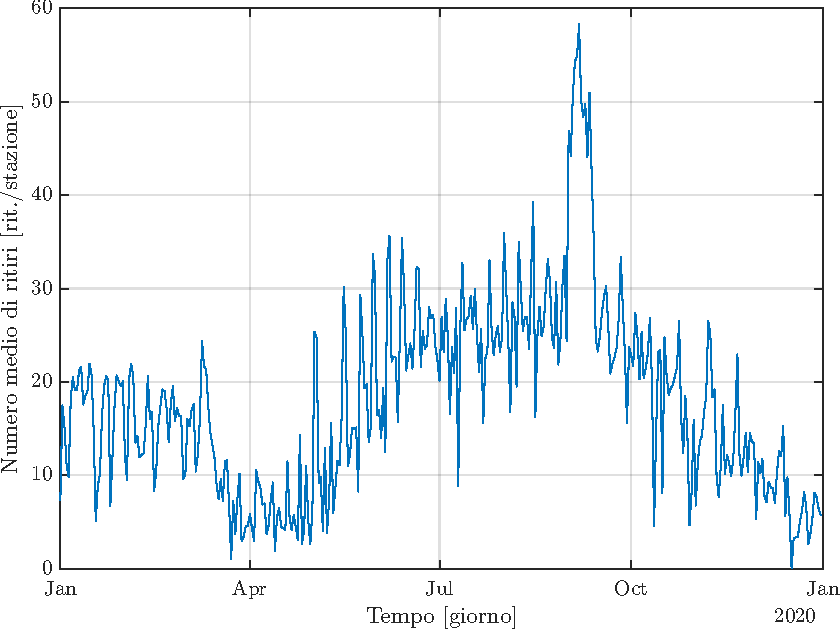
\includegraphics[height=156px]{Immagini/4. Caso di studio/Serie storiche/Ritiri giornalieri}}\quad
	\subfigure[]{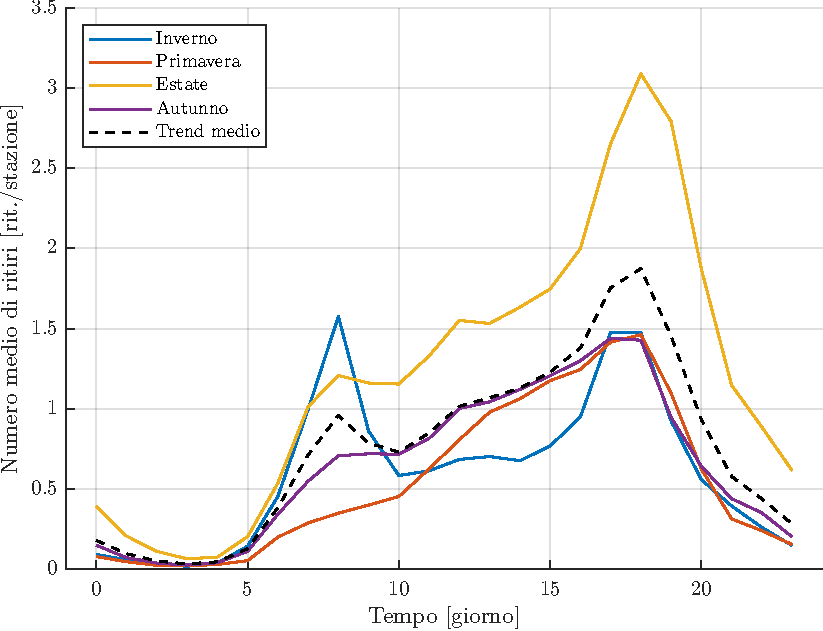
\includegraphics[height=156px]{Immagini/4. Caso di studio/Serie storiche/Ritiri orari}}\quad
	\caption[Andamento giornaliero e orario del numero medio di ritiri al variare della stagione]{andamento giornaliero (a) e orario (b) del numero medio di ritiri al variare della stagione.}
	\label{ritiri_giornalieri_orari}
\end{figure}

\subsection[Variabili meteorologiche]{Variabili meteorologiche}
Le covariate meteorologiche che sono state utilizzate per l'analisi sono:
\begin{itemize}
	\item la \textbf{temperatura percepita}  [\unit{\degreeCelsius}];
	\item la \textbf{pioggia} [\unit{\milli\meter}];
	\item la \textbf{visibilità orizzontale} [\unit{\kilo\meter}];
	\item la \textbf{velocità del vento} [\unit{\kilo\meter/\hour}];
	\item la \textbf{copertura nuvolosa} [\unit{\percent}].
\end{itemize}
Da sottolineare che le variabili sopracitate sono spazio-invarianti e orarie, ovvero sono conseguenza della media eseguita sui campioni rilevati nell'ora da una stazione meteorologica di New York. Inoltre, nella tabella~\ref{statistiche_variabili_meteo} sono riportate le principali statistiche delle covariate in questione; degne di nota la scarsa variabilità della visibilità orizzontale e l'elevata dispersione della copertura nuvolosa nel \num{2020}.

\begin{table}[htp]
	\centering
	\renewcommand\arraystretch{1.5}
	\begin{tabular}{c|c|c|c|c|c|c|c|c}
		\hline
		\textit{Variabile} & \textit{UM} & \textit{Min.} & \textit{Media} & \textit{Med.} & \textit{Mas.} & \textit{Dev.} & \textit{Simm.}  & \textit{Curt.} \\
		\hline
		\textbf{Temp. percep.} & \unit{\degreeCelsius} & \num{-7.66} & \num{13.80} & \num{13.93} & \num{33.33} & \num{9.80} & \num{-0.04} & \num{1.96} \\
		\hline
		\textbf{Pioggia} & \unit{\milli\meter} & \num{0} & \num{1.11} & \num{0} & \num{31.03} & \num{3.44} & \num{5.42} & \num{38.86} \\
		\hline
		\textbf{Visibilità} & \si{\kilo\meter} & \num{6.48} & \num{15.28} & \num{15.99} & \num{16} & \num{1.54} & \num{-2.99} & \num{12.71} \\
		\hline
		\textbf{Vel. del vento} & \si{\kilo\meter/\hour} & \num{4.09} & \num{10.96} & \num{9.81} & \num{27.95} & \num{4.49} & \num{1.34} & \num{4.91} \\
		\hline
		\textbf{Copert. nuvol.} & \si{\percent} & \num{0.08} & \num{39.45} & \num{37.29} & \num{100} & \num{29.71} & \num{0.36} & \num{1.96} \\
		\hline
	\end{tabular}
	\caption[Statistiche principali riguardanti le variabili meteorologiche]{statistiche principali riguardanti le variabili meteorologiche. Per la pioggia è stata eseguita la somma giornaliera.}
	\label{statistiche_variabili_meteo}
\end{table}

\par Infine, è possibile osservare in figura~\ref{ritiri_vs_temperatura} la correlazione positiva esistente tra il numero medio di ritiri giornaliero e la temperatura percepita, mentre in figura~\ref{ritiri_vs_pioggia} l'impatto negativo nei confronti dello stesso da parte della pioggia; nei giorni uggiosi i cittadini newyorkesi prediligono mezzi di trasporto alternativi alla bicicletta.
\par Per gli istogrammi, i box-plot e ulteriori grafici si rimanda all'appendice.

\begin{figure}[htpb]
	\centering
	\subfigure[]{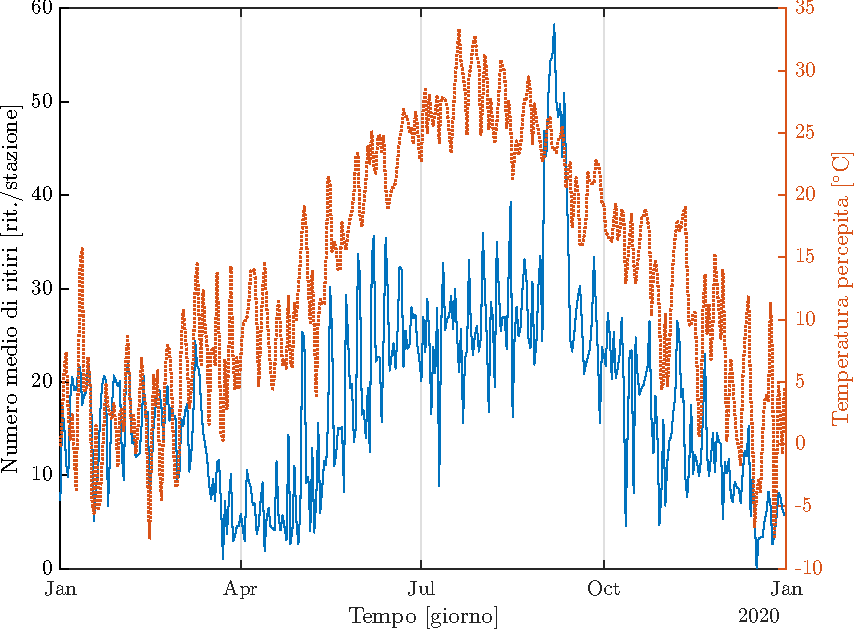
\includegraphics[height=152px]{Immagini/4. Caso di studio/Serie storiche/Ritiri giornalieri e temperatura percepita}\label{ritiri_vs_temperatura}}\quad
	\subfigure[]{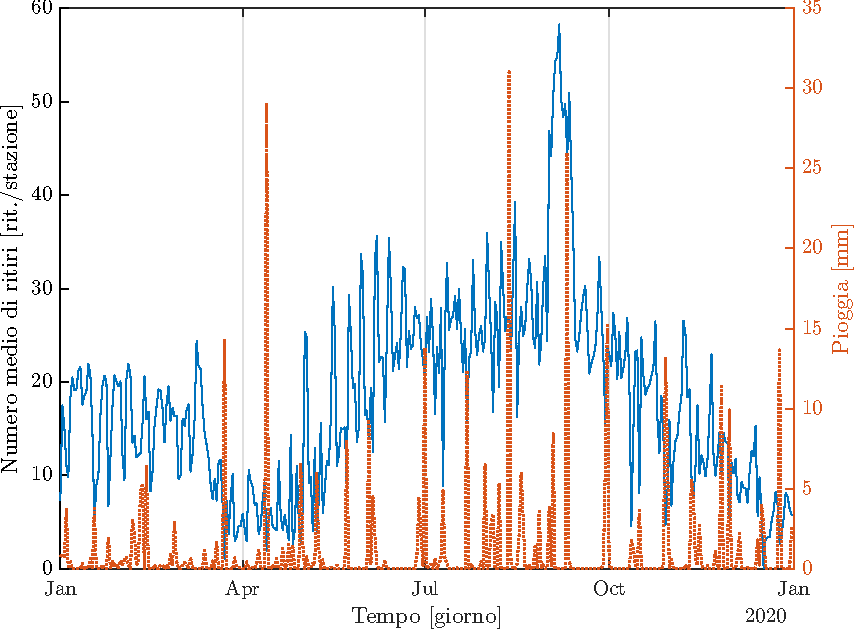
\includegraphics[height=152px]{Immagini/4. Caso di studio/Serie storiche/Ritiri giornalieri e pioggia}\label{ritiri_vs_pioggia}}\quad
	\caption[Confronto tra il numero medio di noleggi giornaliero, la temperatura percepita e la pioggia]{confronto tra il numero medio di noleggi giornaliero, la temperatura percepita (a) e la pioggia (b).}
	\label{ritiri_vs_variabili_meteo}
\end{figure}

\subsection[Variabili spaziali]{Variabili spaziali}
In questa categoria ricadono:
\begin{itemize}
	\item la \textbf{distanza dalla stazione del treno\footnote{o fermata della metropolitana poiché Jersey City è servita da entrambi i mezzi di trasporto pubblico.} più vicina} [\unit{\kilo\meter}];
	\item la \textbf{densità demografica} nella zona alla quale appartiene il punto di ritiro [ab./\unit{\kilo\meter\squared}].
\end{itemize}
Da sottolineare che queste covariate sono spazio-varianti e tempo-invarianti.
\par In figura~\ref{mappa_stazioni_metro} è rappresentata la distanza di ciascun punto di interscambio dalla stazione ferroviaria più vicina. Si osserva una densa concentrazione sia di stazioni ferroviarie che di punti di ritiro delle biciclette nel centro del quartiere, densità che diminuisce man mano che ci si sposta verso le zone limitrofe. Riguardo alla densità demografica, come evidenziato nella figura~\ref{mappa_densita_demografica}, si può notare una distribuzione omogenea su Jersey City. Questa osservazione è supportata dalla ridotta deviazione standard (\num{4278} ab./\unit{\kilo\meter\squared}) della covariata in oggetto (tabella~\ref{statistiche_variabili_spaziali}).

\begin{figure}[htpb]
	\centering
	\subfigure[]{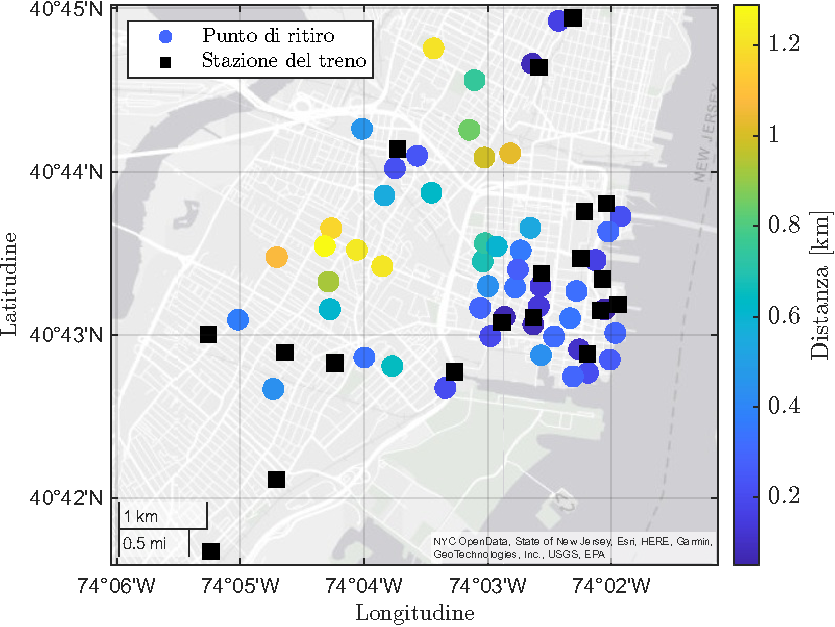
\includegraphics[height=152px]{Immagini/4. Caso di studio/Mappe/Mappa punti ritiro e stazioni treno}\label{mappa_stazioni_metro}}\quad
	\subfigure[]{\includegraphics[height=161px]{Immagini/4. Caso di studio/Mappe/Mappa punti ritiro e densità abitativa}\label{mappa_densita_demografica}}\quad
	\caption[Mappe delle distanze dei punti di interscambio dalla stazione ferroviaria più vicina e della densità abitativa nei pressi dei punti di ritiro]{mappe delle distanze dei punti di interscambio dalla stazione ferroviaria più vicina (a) e della densità abitativa nei pressi dei punti di ritiro (b).}
	\label{mappe_variabili_spaziali}
\end{figure}

\begin{table}[htpb]
	\centering
	\renewcommand\arraystretch{1.5}
	\begin{tabular}{c|c|c|c|c|c|c|c|c}
		\hline
		\textit{Variabile} & \textit{UM} & \textit{Min.} & \textit{Media} & \textit{Med.} & \textit{Mas.} & \textit{Dev.} & \textit{Simm.}  & \textit{Curt.} \\
		\hline
		\textbf{Dist. stazione} & \unit{\kilo\meter} & \num{0.05} & \num{0.49} & \num{0.35} & \num{1.29} & \num{0.36} & \num{0.89} & \num{2.64} \\
		\hline
		\textbf{Dens. dem.} & $\frac{\text{ab.}}{\unit{\kilo\meter\squared}}$ & \num{897} & \num{12215} & \num{11843} & \num{22834} & \num{4278} & \num{-0.15} & \num{2.80} \\
		\hline
	\end{tabular}
	\caption[Statistiche principali riguardanti le variabili spaziali]{statistiche principali riguardanti le variabili spaziali.}
	\label{statistiche_variabili_spaziali}
\end{table} 

\subsection[Variabili dummy]{Variabili dummy}
Alla luce dei risultati ottenuti in~\cite{paper_bike_sharing_Otto}, non solo le condizioni meteorologiche e le covariate spaziali influenzano la domanda giornaliera di noleggi, ma anche altri fattori possono fornire il proprio contributo. In particolare:
\begin{itemize}
	\item il \textbf{lockdown} dovuto alla pandemia di COVID-\num{19};
	\item la successiva \textbf{euforia} dovuta al ritorno alla vita quotidiana dopo mesi trascorsi in isolamento;
	\item i \textbf{weekend} e le \textbf{festività} federali\footnote{giorno di festa ufficialmente riconosciuto a livello federale dal governo degli Stati Uniti.}.
\end{itemize}
Questi eventi sono stati modellati utilizzando \num{3} distinte variabili categoriche binarie (covariate dummy).
\par Infine, la figura~\ref{ritiri_vs_dummy} conferma che, durante la primavera, il numero ridotto di noleggi coincide con il periodo di lockdown, mentre nei weekend si osserva una generale riduzione dell'utilizzo della bicicletta, a dimostrazione che il servizio di bike sharing viene essenzialmente sfruttato nei giorni feriali, probabilmente per i consueti spostamenti lavorativi.

\begin{figure}[htpb]
	\centering
	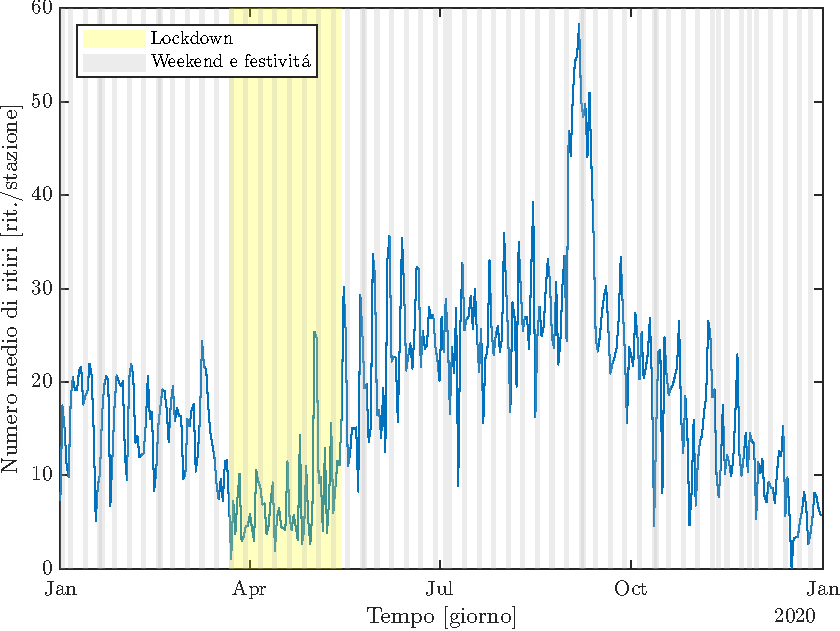
\includegraphics[height=170px]{Immagini/4. Caso di studio/Serie storiche/Ritiri giornalieri e dummy}
	\caption[Confronto tra il numero medio di prelievi giornaliero, il periodo di lockdowwn, i weekend e le festività federali.]{confronto tra il numero medio di prelievi giornaliero, il periodo di lockdowwn, i weekend e le festività federali.}
	\label{ritiri_vs_dummy}
\end{figure}

\section{Sitografia}
\label{sitografia_capitolo_4}
Di seguito sono riportati i riferimenti alle risorse citate in questo capitolo:
\begin{itemize}
	\item \textit{https://climate.copernicus.eu/copernicus-2023-hottest-year-record};
	\item \textit{https://www.kaggle.com/datasets/vineethakkinapalli/citibike-bike-sharingnewyork-cityjan-to-apr-2021};
	\item \textit{https://www.visualcrossing.com/weather-api};
	\item \textit{https://stewartmader.com/subwaynynj/};
	\item \textit{https://sedac.ciesin.columbia.edu/data/set/gpw-v4-population-density-adjusted-to-2015-unwpp-country-totals-rev11};
	\item \textit{https://www.officeholidays.com/countries/usa/new-york/2020};
	\item \textit{https://en.wikipedia.org/wiki/COVID-19\_pandemic\_in\_New\_York\_City}.
\end{itemize}
